\documentclass[12pt, a4paper, oneside, openright, titlepage]{book}
\usepackage[utf8]{inputenc}
\raggedbottom
\usepackage{import}


%%%%%%%%%%%%%%%%% Book Formatting Comments:

%%%%%%%%%%%%%%%%%%%%%%%%%%%%%%%%%%%%% for Part

%%%%%%%%%%%%%%%%%%%%%% for chapter

%%%%%%%%%%%%%%%%%%%% for section








%%%%%% PACKAGES %%%%%%%
\usepackage{hyperref}
\hypersetup{
    colorlinks,
    citecolor=black,
    filecolor=black,
    linkcolor=black,
    urlcolor=black
}
\usepackage{amsmath} % Math display options
\usepackage{amssymb} % Math symbols
\usepackage{amsfonts} % Math fonts
\usepackage{amsthm}
\usepackage{mathtools} % General math tools
\usepackage{array} % Allows you to write arrays
\usepackage{empheq} % For boxing equations
\usepackage{mathabx}
\usepackage{mathrsfs}
\usepackage{nameref}

\usepackage{soul}
\usepackage[normalem]{ulem}

\usepackage{txfonts}
\usepackage{cancel}
\usepackage[toc, page]{appendix}
\usepackage{titletoc,tocloft}
\setlength{\cftchapindent}{1em}
\setlength{\cftsecindent}{2em}
\setlength{\cftsubsecindent}{3em}
\setlength{\cftsubsubsecindent}{4em}
\usepackage{titlesec}

\titleformat{\section}
  {\normalfont\fontsize{25}{15}\bfseries}{\thesection}{1em}{}
\titleformat{\section}
  {\normalfont\fontsize{20}{15}\bfseries}{\thesubsection}{1em}{}
\setcounter{secnumdepth}{1}  
  
  

\newcommand\numberthis{\refstepcounter{equation}\tag{\theequation}} % For equation labelling
\usepackage[framemethod=tikz]{mdframed}

\usepackage{tikz} % For drawing commutative diagrams
\usetikzlibrary{cd}
\usetikzlibrary{calc}
\tikzset{every picture/.style={line width=0.75pt}} %set default line width to 0.75p

\usepackage{datetime}
\usepackage[margin=1in]{geometry}
\setlength{\parskip}{1em}
\usepackage{graphicx}
\usepackage{float}
\usepackage{fancyhdr}
\setlength{\headheight}{15pt} 
\pagestyle{fancy}
\lhead[\leftmark]{}
\rhead[]{\leftmark}

\usepackage{enumitem}

\usepackage{url}
\allowdisplaybreaks

%%%%%% ENVIRONMENTS %%%
\definecolor{purp}{rgb}{0.29, 0, 0.51}
\definecolor{bloo}{rgb}{0, 0.13, 0.80}



%%\newtheoremstyle{note}% hnamei
%{3pt}% hSpace above
%{3pt}% hSpace belowi
%{}% hBody fonti
%{}% hIndent amounti
%{\itshape}% hTheorem head fonti
%{:}% hPunctuation after theorem headi
%{.5em}% hSpace after theorem headi
%{}% hTheorem head spec (can be left empty, meaning ‘normal’)i


%%%%%%%%%%%%% THEOREM STYLES

\newtheoremstyle{BigTheorem}
{20pt}
{20pt}
{\slshape}
{}
{\Large\color{purp}\bfseries}
{.}
{\newline}
{\thmname{#1}\thmnumber{ #2}\thmnote{ (#3)}}



\newtheoremstyle{TheoremClassic}
{15pt}
{15pt}
{\slshape}
{}
{\bfseries}
{.}
{.5em}
{}

\newtheoremstyle{Definitions}
{15pt}
{15pt}
{\slshape}
{}
{\bfseries}
{.}
{.5em}
{\thmname{#1}\thmnumber{ #2}\thmnote{ (#3)}}


\newtheoremstyle{Remarks}
{10pt}
{10pt}
{\upshape}
{}
{\bfseries}
{.}
{.5em}
{}

\newtheoremstyle{Examples}
{10pt}
{10pt}
{\upshape}
{}
{\bfseries}
{.}
{.5em}
{}


%%%%%%%%%%%%% THEOREM DEFINITIONS

\theoremstyle{BigTheorem}
\newtheorem{namthm}{Theorem}
\newtheorem{conj}[namthm]{Conjecture}

\theoremstyle{TheoremClassic}
\newtheorem{thm}{Theorem}[section]
\newtheorem*{thm*}{Theorem}
\newtheorem{lem}[thm]{Lemma}
\newtheorem{cor}[thm]{Corollary}
\newtheorem{prop}[thm]{Proposition}
\newtheorem{claim}[thm]{Claim}


\theoremstyle{Definitions}
\newtheorem{defn}{Definition}[section]
\newtheorem{axi}[defn]{Axiom}
\newtheorem{cust}[defn]{}
\newtheorem{cons}[defn]{Construction}
\newtheorem{props}[defn]{Properties}
\newtheorem{proc}[defn]{Process}
\newtheorem*{law}{Law}


\theoremstyle{Examples}
\newtheorem{eg}{Example}[section]
\newtheorem{noneg}[eg]{Non-Example}
\newtheorem{xca}[eg]{Exercise}


\theoremstyle{Remarks}
\newtheorem{rmk}{Remark}[section]
\newtheorem{qst}[rmk]{Question}
\newtheorem*{ans}{Answer}
\newtheorem{obs}[rmk]{Observation}
\newtheorem{rec}[rmk]{Recall}
\newtheorem{summ}[rmk]{Summary}
\newtheorem{nota}[rmk]{Notation}
\newtheorem{note}[rmk]{Note}



\renewcommand{\qedsymbol}{$\blacksquare$}


\numberwithin{equation}{section}

\newenvironment{qest}{
    \begin{center}
        \em
    }
    {
    \end{center}
    }

%%%%%% MACROS %%%%%%%%%
%% New Commands
\newcommand{\ip}[1]{\langle#1\rangle} %%% Inner product
\newcommand{\abs}[1]{\lvert#1\rvert} %%% Modulus
\newcommand\diag{\operatorname{diag}} %%% diag matrix
\newcommand\tr{\mbox{tr}\.} %%% trace
\newcommand\C{\mathbb C} %%% Complex numbers
\newcommand\R{\mathbb R} %%% Real numbers
\newcommand\Z{\mathbb Z} %%% Integers
\newcommand\Q{\mathbb Q} %%% Rationals
\newcommand\N{\mathbb N} %%% Naturals
\newcommand\F{\mathbb F} %%% An arbitrary field
\newcommand\ste{\operatorname{St}} %%% Steinberg Representation
\newcommand\GL{\mathbf{GL}} %%% General Linear group
\newcommand\SL{\mathbf{SL}} %%% Special linear group
\newcommand\gl{\mathfrak{gl}} %%% General linear algebra
\newcommand\G{\mathbf{G}} %%% connected reductive group
\newcommand\g{\mathfrak{g}} %%% Lie algebra of G
\newcommand\Hbf{\mathbf{H}} %%% Theta fixed points of G
\newcommand\X{\mathbf{X}} %%% Symmetric space X
\newcommand{\catname}[1]{\normalfont\textbf{#1}}
\newcommand{\Set}{\catname{Set}} %%% Category set
\newcommand{\Grp}{\catname{Grp}} %%% Category group
\newcommand{\Rmod}{\catname{R-Mod}} %%% Category r-modules
\newcommand{\Mon}{\catname{Mon}} %%% Category monoid
\newcommand{\Ring}{\catname{Ring}} %%% Category ring
\newcommand{\Topp}{\catname{Top}} %%% Category Topological spaces
\newcommand{\Vect}{\catname{Vect}_{k}} %%% category vector spaces'
\newcommand\Hom{\mathbf{Hom}} %%% Arrows

\newcommand{\map}[2]{\begin{array}{c} #1 \\ #2 \end{array}}

\newcommand{\Emph}[1]{\textbf{\ul{\emph{#1}}}}

\newcommand{\mapsfrom}{\mathrel{\reflectbox{\ensuremath{\mapsto}}}}


%% Math operators
\DeclareMathOperator{\ran}{Im} %%% image
\DeclareMathOperator{\aut}{Aut} %%% Automorphisms
\DeclareMathOperator{\spn}{span} %%% span
\DeclareMathOperator{\ann}{Ann} %%% annihilator
\DeclareMathOperator{\rank}{rank} %%% Rank
\DeclareMathOperator{\ch}{char} %%% characteristic
\DeclareMathOperator{\ev}{\bf{ev}} %%% evaluation
\DeclareMathOperator{\sgn}{sign} %%% sign
\DeclareMathOperator{\id}{Id} %%% identity
\DeclareMathOperator{\supp}{Supp} %%% support
\DeclareMathOperator{\inn}{Inn} %%% Inner aut
\DeclareMathOperator{\en}{End} %%% Endomorphisms
\DeclareMathOperator{\sym}{Sym} %%% Group of symmetries


%% Diagram Environments
\iffalse
\begin{center}
    \begin{tikzpicture}[baseline= (a).base]
        \node[scale=1] (a) at (0,0){
          \begin{tikzcd}
           
          \end{tikzcd}
        };
    \end{tikzpicture}
\end{center}
\fi




\newdateformat{monthdayyeardate}{%
    \monthname[\THEMONTH]~\THEDAY, \THEYEAR}
%%%%%%%%%%%%%%%%%%%%%%%

%%% Specific Macros %%%


%%%%%% BEGIN %%%%%%%%%%


\begin{document}

%%%%%% TITLE PAGE %%%%%

\begin{titlepage}
    \centering
    \scshape
    \vspace*{\baselineskip}
    \rule{\textwidth}{1.6pt}\vspace*{-\baselineskip}\vspace*{2pt}
    \rule{\textwidth}{0.4pt}
    
    \vspace{0.75\baselineskip}
    
    {\LARGE Statistical Mechanics: A Complete Guide}
    
    \vspace{0.75\baselineskip}
    
    \rule{\textwidth}{0.4pt}\vspace*{-\baselineskip}\vspace{3.2pt}
    \rule{\textwidth}{1.6pt}
    
    \vspace{2\baselineskip}
    Phys 449 \\
    \vspace*{3\baselineskip}
    \monthdayyeardate\today \\
    \vspace*{5.0\baselineskip}
    
    {\scshape\Large Elijah Thompson, \\ Physics and Math Honors\\}
    
    \vspace{1.0\baselineskip}
    \textit{Solo Pursuit of Learning}
    \vfill
    \enlargethispage{1in}
    \begin{figure}[b!]
    \makebox[\textwidth]{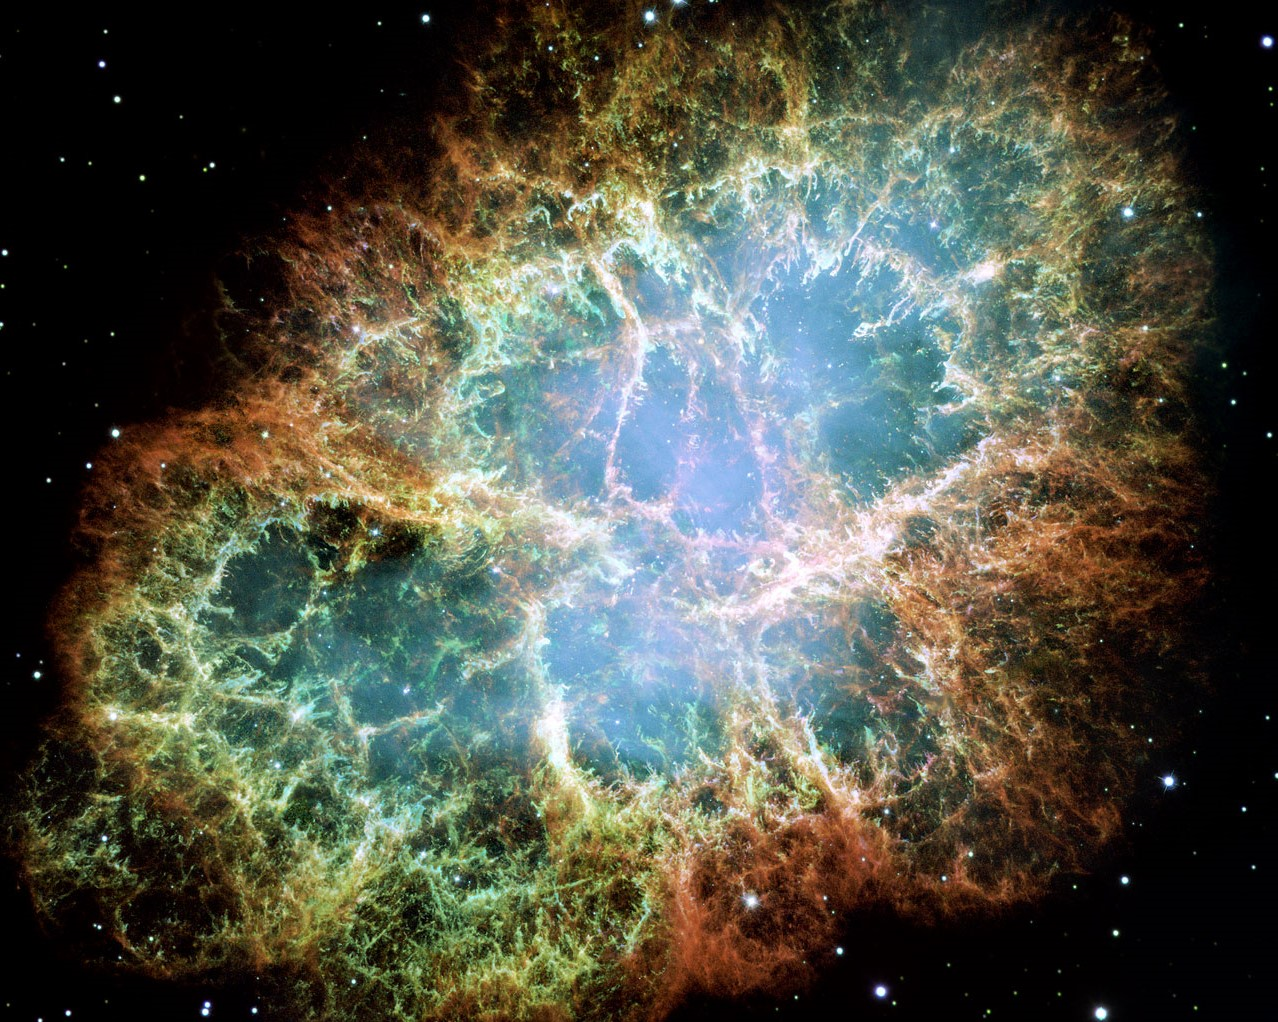
\includegraphics[width=\paperwidth, height =10cm]{../Crab.jpg}}
    \end{figure}
\end{titlepage}

%%%%%%%%%%%%%%%%%%%%%%%
\tableofcontents



%%%%%%%%%%%%%%%%%%%%%%%%%%%%%%%%%%%%% Part 1
\part{Thermodynamics}

%%%%%%%%%%%%%%%%%%%%%% Chapter 1.1
\chapter{Energy in Thermal Physics}

%%%%%%%%%%%%%%%%%%%% Section 1.1.1
\section{Basic Notation and Work}

\begin{defn}
    Thermodynamics is a \Emph{phenomenological} description of properties of \Emph{macroscopic systems} in \Emph{thermal equilibrium}.
\end{defn}

By a phenomenological description we mean a discription based on observations and direct experience of the experimenter with the system, considered as a ``black box" (a system whose internal structure is unknown, or is just not considered). The task of thermodynamics is to define appropriate physical quanitities, \Emph{state quantities}, which characterize macroscopic properties of matter, that is \Emph{macrostates}, in a way which is as unambiguous as possible, and to relate these quantities by means of universally valid equations.

\begin{defn}[Systems]
    There are a number of different thermodynamic systems. In particular we define a thermodynamic system, in general, to be an arbitrary amount of matter, the properties of which can be uniquely and completely described by specifying certain macroscopic parameters. We summarize them as follows: \begin{itemize}
        \item \Emph{Thermodynamic or Macroscopic System:} A system consisting of a large number of constituents. For example, a mole of gas (approximately $10^{23}$ particles) can be considered as a macroscopic system.
        \item \Emph{Isolated Thermodynamic System:} A system which exhibits no exchange of any type with the surroundings; no exchange of work, heat, matter, etc. The total energy (mechanical, electrical, etc.) is a conserved quantity for such a system, and can thus be used to characterize the macrostate.
        \item \Emph{Closed Theormodynamic System:} A system which exhibits no exchange of matter with its surroundings. Hence, energy exchange is allowed, so energy is no longer a conserved quantity and can fluctuate due to exchange with the surroundings. The termperature, particle number, and volume of the system can characterize the macrostate.
        \item \Emph{Open Thermodynamic System:} A system for which it is possible for exchange of any type with the surroundings (work, heat, matter, etc.). Energy and particle number are both not conserved. But, temperature and chemical potential can still be used to characterize a macrostate.
    \end{itemize}
\end{defn}

If the properties of a system are the same for any part of it, one calls such a system \Emph{homogeneous}. On the other hand, if the properties change discontinuously at certain marginal surfaces, the system is \Emph{heterogeneous}, with the homogeneous portions of the system called \Emph{phases} and the separating surfaces \Emph{phase boundaries}. 

\begin{defn}
    The macroscopic quantities which describe a system are called state quantities.
\end{defn}

\begin{eg}
    Examples of state quantities are the system's energy $E$, its volume $V$, its particle number $N$, its entropy $S$, its temperature $T$, the pressure $P$, the chemical potential $\mu$, the charge $q$, the dipole momentum, the refractive index, the viscosity, the chemical composition, and the size of phase boundaries.
\end{eg}

However, microscopic quantities do not fall under the umbrella of state quantities.

\begin{defn}[Equilibrium]
    Two thermodynamic systems are in \Emph{equilibrium} if and only if they are in contact such that they can exchange a given conserved quantity (for example particles) and they are relaxed to a state in which there is no average net transfer of that quantity between them anymore. A thermodynamic system $S$ is in equilibrium with itself, if and only if, all its subsystems are in equilibrium with each other. In this case, $S$ is called an \Emph{equilibrium} system.
\end{defn}

From this definition we find that different types of exchanged quanitities can lead to different types of equilibria: 

\begin{table}[H]
    \centering
    \begin{tabular}{c|c}
        \hline
        Exchanged Quantity & Type of Equilibrium \\ \hline \hline
        Particles/Matter & Diffusive Equilibrium \\ 
        Work & Mechanical Equilibrium \\
        Heat & Thermal Equilibrium \\ \hline
    \end{tabular}
\end{table}

\begin{defn}
    \Emph{Complete Thermodynamic Equilibrium} corresponds to a state where all the conserved fluxes between two coupled thermodynamic systems vanish.
\end{defn}

A way of testing if a given system is in a complete thermodynamic equilibrium is if the properties of the system do not change appreciably over the observation time, which is to say the properties reflect the true asymptotic long-term properties after any initial relaxation time is over.

The state of thermodynamic systems in complete thermodynamic equilibrium can be described by a set of independent \Emph{thermodynamic coordinates} or \Emph{state variables}; this fact is based on empirical observations. 

\subsection{Boyle-Mariotte's Experiment}

\begin{law}
    For a given mass of gas at a constant temperature $T$, the volume $V$ is inverseley proportional to the pressure $P$: $V \propto P^{-1}$.
\end{law}

We consider Robert Boyle's (1627-1691) experiment, conducted at room temperature, which should remain constant during the time of the experiment. We use a vertical tube with markings to indicate the volume of gas, and oil at the bottom. By applying pressure on the oil, we also exert a pressure on the air in the tube above the oil, causing the volume to decrease. Drawing the graph of volume versus $P^{-1}$ we obtain a straight line, so $V\cdot P = C$ for some constant $C$, given a fixed temperature. As further measurements show, the constant is proportional to the temperature $T$, so $V\cdot P \propto T$. More precisely, the full equation of a state of simple low-density gase is given by \begin{equation}
    \boxed{PV = Nk_BT}
\end{equation}
where $N$ is the number of gas particles and $k_B \approx 1.381\times 10^{-23}\;J/K$ is a natural constant called the \Emph{Boltzmann's constant}. The above equation is called the \Emph{ideal gas law} or the \Emph{equation of state for an ideal gas} since it relates the three state variables, or thermodynamic coordinates, $P$, $V$, and $T$ at equilibrium.

\subsubsection{Mechanical Derivation}

We now sketch a derivation of the ideal gas law using an atomistic theory governed by Newton's Laws. First assume there is a single molecule or atom bouncing around in a volume $V = AL$, where $L$ is the length along the $x$-direction and $A$ is the area of a side parallel to the $yz$-plane:

\begin{center}
    \begin{tikzpicture}[x=0.75pt,y=0.75pt,yscale=-1.4,xscale=1.4]
%uncomment if require: \path (0,398); %set diagram left start at 0, and has height of 398

%Shape: Cube [id:dp41058044355698486] 
\draw   (130,134) -- (154,110) -- (240,110) -- (240,166) -- (216,190) -- (130,190) -- cycle ; \draw   (240,110) -- (216,134) -- (130,134) ; \draw   (216,134) -- (216,190) ;
%Straight Lines [id:da3652266253176417] 
\draw    (132,200) -- (208,200) ;
\draw [shift={(210,200)}, rotate = 180] [color={rgb, 255:red, 0; green, 0; blue, 0 }  ][line width=0.75]    (6.56,-1.97) .. controls (4.17,-0.84) and (1.99,-0.18) .. (0,0) .. controls (1.99,0.18) and (4.17,0.84) .. (6.56,1.97)   ;
\draw [shift={(130,200)}, rotate = 0] [color={rgb, 255:red, 0; green, 0; blue, 0 }  ][line width=0.75]    (6.56,-1.97) .. controls (4.17,-0.84) and (1.99,-0.18) .. (0,0) .. controls (1.99,0.18) and (4.17,0.84) .. (6.56,1.97)   ;
%Straight Lines [id:da08447016298808463] 
\draw    (166.89,172.06) -- (190.59,155.21) ;
\draw [shift={(192.22,154.06)}, rotate = 504.61] [color={rgb, 255:red, 0; green, 0; blue, 0 }  ][line width=0.75]    (6.56,-1.97) .. controls (4.17,-0.84) and (1.99,-0.18) .. (0,0) .. controls (1.99,0.18) and (4.17,0.84) .. (6.56,1.97)   ;
%Curve Lines [id:da14521036207082538] 
\draw    (268.22,143.72) .. controls (250.49,160.14) and (256.69,125.13) .. (232.99,150.84) ;
\draw [shift={(231.89,152.06)}, rotate = 311.76] [color={rgb, 255:red, 0; green, 0; blue, 0 }  ][line width=0.75]    (6.56,-1.97) .. controls (4.17,-0.84) and (1.99,-0.18) .. (0,0) .. controls (1.99,0.18) and (4.17,0.84) .. (6.56,1.97)   ;
%Straight Lines [id:da5265921627377463] 
\draw  [dash pattern={on 0.84pt off 2.51pt}]  (130,190) -- (141.22,190) ;
\draw [shift={(143.22,190)}, rotate = 180] [color={rgb, 255:red, 0; green, 0; blue, 0 }  ][line width=0.75]    (4.37,-1.32) .. controls (2.78,-0.56) and (1.32,-0.12) .. (0,0) .. controls (1.32,0.12) and (2.78,0.56) .. (4.37,1.32)   ;
%Straight Lines [id:da8512625721822618] 
\draw  [dash pattern={on 0.84pt off 2.51pt}]  (130,190) -- (137.8,182.35) ;
\draw [shift={(139.22,180.94)}, rotate = 495.52] [color={rgb, 255:red, 0; green, 0; blue, 0 }  ][line width=0.75]    (4.37,-1.32) .. controls (2.78,-0.56) and (1.32,-0.12) .. (0,0) .. controls (1.32,0.12) and (2.78,0.56) .. (4.37,1.32)   ;
%Straight Lines [id:da2755149870872269] 
\draw  [dash pattern={on 0.84pt off 2.51pt}]  (130,190) -- (130,181.94) ;
\draw [shift={(130,179.94)}, rotate = 450] [color={rgb, 255:red, 0; green, 0; blue, 0 }  ][line width=0.75]    (4.37,-1.32) .. controls (2.78,-0.56) and (1.32,-0.12) .. (0,0) .. controls (1.32,0.12) and (2.78,0.56) .. (4.37,1.32)   ;

% Text Node
\draw (167,198) node [anchor=north west][inner sep=0.75pt]  [font=\scriptsize,color={rgb, 255:red, 255; green, 0; blue, 0 }  ,opacity=1 ]  {$L$};
% Text Node
\draw (166.89,172.06) node [anchor=center][inner sep=0.75pt]  [font=\LARGE,color={rgb, 255:red, 255; green, 0; blue, 0 }  ,opacity=1 ]  {$\cdot $};
% Text Node
\draw (170.56,151.96) node [anchor=north west][inner sep=0.75pt]  [font=\scriptsize,color={rgb, 255:red, 255; green, 0; blue, 0 }  ,opacity=1 ]  {$\vec{v}$};
% Text Node
\draw (269.56,135.96) node [anchor=north west][inner sep=0.75pt]  [font=\scriptsize,color={rgb, 255:red, 255; green, 0; blue, 0 }  ,opacity=1 ]  {$A$};
% Text Node
\draw (142.56,189.84) node [anchor=north west][inner sep=0.75pt]  [font=\tiny]  {$x$};
% Text Node
\draw (140.89,176.51) node [anchor=north west][inner sep=0.75pt]  [font=\tiny]  {$y$};
% Text Node
\draw (124.89,173.84) node [anchor=north west][inner sep=0.75pt]  [font=\tiny]  {$z$};


\end{tikzpicture}
\end{center}

After many perfectly ellastic collisions against the wall, the average pressure directly on the wall is \begin{equation*}
    \overline{p} = \frac{\overline{F}_{x,on\;wall}}{A} = -\frac{\overline{F}_{x,on\;molecule}}{A} = -\frac{m\overline{\frac{\Delta v_x}{\Delta t}}}{A} 
\end{equation*}
The time it takes for a full round trip is $\Delta t = 2L/v_x$. When it undergoes one elastic collision, its change in velocity is $\Delta v_x = -2v_x$. Together these give \begin{equation*}
    \overline{p} = -\frac{m(-2v_x/(2L/v_x))}{A} = \frac{mv_x^2}{LA} = \frac{mv_x^2}{V}
\end{equation*}
Now, if we extend to $N >> 1$ non-interacting molecules, each colliding with the walls totally elastically, then we can forgoe the averageness of the pressure to obtain \begin{equation*}
    pV = m\sum_{i=1}^N(v_x^2)_i = mN\overline{v_x^2} = Nk_BT
\end{equation*}
using the ideal gas law at the end, which gives the relation \begin{equation*}
    \overline{K}_x = \overline{\frac{1}{2}mv_x^2} = \frac{1}{2}k_BT
\end{equation*}
Then we find that the total mean kinetic energy is \begin{equation}
    \overline{K} = \frac{1}{2}m\overline{v_x^2}+\frac{1}{2}m\overline{v_y^2}+\frac{1}{2}m\overline{v_z^2} = \frac{3}{2}k_BT
\end{equation}

\begin{defn}
    The \Emph{Root-mean square speed} of each atom/molecule is defined as \begin{equation*}
        v_{RMS} = \sqrt{\overline{v^2}}
    \end{equation*}
\end{defn}

In general the RMS speed is often a close approximation of the average speed. In this case we have $v_{RMS} = \sqrt{3k_BT/m}$.


\subsection{Work}

\begin{defn}
    Given a vector force field $\vec{F}$ defined along a path $\gamma$, the \Emph{work} $W$ is of $\vec{F}$ along $\gamma$ is defined to be: \begin{equation}
        W = \int_{\gamma}\vec{F}\cdot d\vec{r}
    \end{equation}
\end{defn}

\begin{rec}
    Recall that pressure is force per unit area, so we have that \begin{equation*}
        P = \frac{F}{A}
    \end{equation*}
    where $F$ is the normal component of the force to the area $A$. More precisely, pressure is the proportionality constant that relates the force and normal vectors: \begin{equation*}
        d\vec{F}_n = -pd\vec{A}
    \end{equation*}
    where $\vec{F}_n$ denotes the normal component of the force vector $\vec{F}$.
\end{rec}


\begin{eg}
    Consider the compression of a gas by a piston with a constant force of magnitude $F$.
    \begin{center}
    \begin{tikzpicture}[x=0.75pt,y=0.75pt,yscale=-1.2,xscale=1.2]
%uncomment if require: \path (0,398); %set diagram left start at 0, and has height of 398

%Shape: Rectangle [id:dp9125760638904235] 
\draw   (100,110) -- (200,110) -- (200,160) -- (100,160) -- cycle ;
%Straight Lines [id:da19743423815417427] 
\draw    (200,110) -- (230,110) ;
%Straight Lines [id:da17599416360044806] 
\draw    (200,160) -- (230,160) ;
%Straight Lines [id:da37025754978607806] 
\draw [color={rgb, 255:red, 255; green, 27; blue, 0 }  ,draw opacity=1 ]   (200,110) -- (200,160) ;
%Straight Lines [id:da5752016333947421] 
\draw [color={rgb, 255:red, 255; green, 27; blue, 0 }  ,draw opacity=1 ]   (200,135) -- (250,135) ;
%Straight Lines [id:da4588247522685671] 
\draw    (230,127) -- (222,127) ;
\draw [shift={(220,127)}, rotate = 360] [color={rgb, 255:red, 0; green, 0; blue, 0 }  ][line width=0.75]    (4.37,-1.32) .. controls (2.78,-0.56) and (1.32,-0.12) .. (0,0) .. controls (1.32,0.12) and (2.78,0.56) .. (4.37,1.32)   ;
%Curve Lines [id:da22459360243367987] 
\draw [line width=0.75]    (281.89,123.39) .. controls (280.27,107.22) and (224.4,110.81) .. (204.92,121.69) ;
\draw [shift={(203.22,122.72)}, rotate = 326.56] [color={rgb, 255:red, 0; green, 0; blue, 0 }  ][line width=0.75]    (6.56,-1.97) .. controls (4.17,-0.84) and (1.99,-0.18) .. (0,0) .. controls (1.99,0.18) and (4.17,0.84) .. (6.56,1.97)   ;
%Straight Lines [id:da04861500853364609] 
\draw    (200,170) -- (192,170) ;
\draw [shift={(190,170)}, rotate = 360] [color={rgb, 255:red, 0; green, 0; blue, 0 }  ][line width=0.75]    (4.37,-1.32) .. controls (2.78,-0.56) and (1.32,-0.12) .. (0,0) .. controls (1.32,0.12) and (2.78,0.56) .. (4.37,1.32)   ;
%Straight Lines [id:da2692578781738837] 
\draw    (200,167) -- (200,173) ;

% Text Node
\draw (231,122.4) node [anchor=north west][inner sep=0.75pt]  [font=\tiny,color={rgb, 255:red, 246; green, 12; blue, 12 }  ,opacity=1 ]  {$\vec{F}$};
% Text Node
\draw (237,125) node [anchor=north west][inner sep=0.75pt]  [font=\tiny] [align=left] {(const.)};
% Text Node
\draw (270.89,125.89) node [anchor=north west][inner sep=0.75pt]  [font=\tiny] [align=left] {Piston area:};
% Text Node
\draw (311.89,125.4) node [anchor=north west][inner sep=0.75pt]  [font=\tiny,color={rgb, 255:red, 255; green, 0; blue, 0 }  ,opacity=1 ]  {$\mathcal{A}$};
% Text Node
\draw (108.56,114.4) node [anchor=north west][inner sep=0.75pt]  [font=\small]  {$\cdot $};
% Text Node
\draw (128.56,134.4) node [anchor=north west][inner sep=0.75pt]  [font=\small]  {$\cdot $};
% Text Node
\draw (128.56,134.4) node [anchor=north west][inner sep=0.75pt]  [font=\small]  {$\cdot $};
% Text Node
\draw (139.89,121.07) node [anchor=north west][inner sep=0.75pt]  [font=\small]  {$\cdot $};
% Text Node
\draw (159.89,141.07) node [anchor=north west][inner sep=0.75pt]  [font=\small]  {$\cdot $};
% Text Node
\draw (127.56,112.07) node [anchor=north west][inner sep=0.75pt]  [font=\small]  {$\cdot $};
% Text Node
\draw (161.56,117.4) node [anchor=north west][inner sep=0.75pt]  [font=\small]  {$\cdot $};
% Text Node
\draw (181.56,137.4) node [anchor=north west][inner sep=0.75pt]  [font=\small]  {$\cdot $};
% Text Node
\draw (110.22,132.4) node [anchor=north west][inner sep=0.75pt]  [font=\small]  {$\cdot $};
% Text Node
\draw (179.22,114.73) node [anchor=north west][inner sep=0.75pt]  [font=\small]  {$\cdot $};
% Text Node
\draw (142.89,141.4) node [anchor=north west][inner sep=0.75pt]  [font=\small]  {$\cdot $};
% Text Node
\draw (168.22,127.73) node [anchor=north west][inner sep=0.75pt]  [font=\small]  {$\cdot $};
% Text Node
\draw (148.22,112.73) node [anchor=north west][inner sep=0.75pt]  [font=\small]  {$\cdot $};
% Text Node
\draw (123.56,124.07) node [anchor=north west][inner sep=0.75pt]  [font=\small]  {$\cdot $};
% Text Node
\draw (111.56,142.73) node [anchor=north west][inner sep=0.75pt]  [font=\small]  {$\cdot $};
% Text Node
\draw (192,173.4) node [anchor=north west][inner sep=0.75pt]  [font=\tiny]  {$\Delta x$};


\end{tikzpicture}
\end{center}
    so the work is \begin{equation*}
        W = \int_{\gamma}\vec{F}\cdot d\vec{r} = F\int_{\gamma}dr = F\Delta x = PA\Delta x = -P\Delta V
    \end{equation*}
    where $P$ is the pressure and $\Delta V$ is the change in volume. Since the change in volume is negative, the work $W$ done on the system (here the gas) is positive: Energy is added to the system by a force (macroscopic) process (here the piston). $W< 0$ if energy is removed from the system.
\end{eg}


\begin{defn}
    The generalized differential form for work is given by \begin{equation}
        \delta W = \sum_{i=1}^mJ_idq_i
    \end{equation}
    where $q_i$ are the generalized coordinates and the $J_i$ are the conjugate generalized forces such that $J_idq_i$ has units of energy. This is possible when the system is undergoing an infinitesimal quasi-static transformation.
\end{defn}

Here are a few examples of generalized coordinates and their corresponding generalized conjugate forces:

\begin{table}[H]
    \centering
    \begin{tabular}{c|c|c}
        \hline
        & Generalized Force $J_i$ & Generalized Coordinate $dq_i$ \\ \hline \hline
        Pressure & $-P$ & $dV$ (change in volume) \\ 
        Surface tension & $\sigma$ & $dS$ (change in surface area) \\
        Magnetic field & $\vec{B}_0$ & $d\vec{m}$ (change in magnetic moment) \\
        Electric field & $\vec{E}$ & $d\vec{P}$ (change in electric dipole moment) \\\hline
    \end{tabular}
\end{table}

\begin{defn}
    Differential changes in a systems property are said to be \Emph{quasi-static} if the changes occur on time scales much longer than the relaxation time such that the system remains in equilibrium at all times.
\end{defn}

To ensure thermodynamics is a self-consistent description of macroscopic systems in thermal equilibrium we must assume that the differential changes $\delta W$ are quasi-static. This also ensures that we can describe the state of such a thermodynamic system by a set of thermodynamic coordinates at all times, which is to state at any stage of the process the thermodynamic coordinates of the system exist and can in principle be computed. 

Depending on the macroscopic generalized force, the work necessary to transfer a thermodynamic system in complete thermodynamic equilibrium from state $A$ to state $B$ might or might not depend on the path taken. For example, if $\gamma_1$ and $\gamma_2$ are two paths from state $A$ to state $B$, it is possible that $\int_{\gamma_1}\delta W \neq \int_{\gamma_2}\delta W$. (Note that this justifies the use of the notation $\delta W$ over $dW$, which would denote an exact differential)


\begin{defn}
    State quantities which are proportional to the amount of matter in a system are called \Emph{extensive}, and are consequently additive when looking at subsystems.
\end{defn}

\begin{defn}
    State quantities which are independent of the amount of matter in the system are called \Emph{intensive}, and are not additive for the particular phases of the system.
\end{defn}

Intensive quantities are indicators of equilibrium. 


\subsection{Conservative Forces}

\begin{rec}
    Recall that a conservative force is a force $\vec{F}$ with an associated potential energy function $E$ such that $\vec{F} = \nabla E$.
\end{rec}

\begin{prop}
    If the macroscopic generalized force $\vec{J}$, depending on $m$ generalized coordinates $q_i$, is conservative with potential energy $E_{pot}$ which is twice continuously differentiable and the domain of integration is simply connected, then the following are equivalent:
    \begin{itemize}
        \item $\vec{J}(\vec{q}) = -\nabla E_{pot}(\vec{q})$
        \item $dW$ is an exact differential form, so $$\int_{\gamma}dW = \int_{\gamma}\vec{J}\cdot d\vec{r}$$ depends only on the endpoints of $\gamma$.
        \item For any simple closed path $\gamma$, $$\oint_{\gamma}dW = \oint_{\gamma}\vec{J}\cdot d\vec{r} = 0$$
        \item The curl of $\vec{J}$ is trivial over the domain of integration $$\nabla \times \vec{J} = 0$$ provided that $m = 3$
        \item For all $i,j \in \{1,2,...,m\}$, we have that \begin{equation*}
                \frac{\partial J_i}{\partial q_j} - \frac{\partial J_j}{\partial q_i} = 0
        \end{equation*}
        \item The differential $dW$ is exact, and we have that \begin{equation*}
                dW = -\nabla E_{pot}\cdot d\vec{r} = -\sum_{i=1}^m\frac{\partial E_{pot}}{\partial q_i}dq_i = -dE_{pot}
        \end{equation*}
    \end{itemize}
\end{prop}


\begin{defn}
    For a function $A(q_1,q_2,...,q_m)$ the \Emph{total differential} or \Emph{exact differential} of $A$ is given by \begin{equation*}
        dA = \sum_{i=1}^m\frac{\partial A}{\partial q_i}dq_i
    \end{equation*}
    This corresponds to a generalized chain rule: \begin{equation*}
        \frac{dA}{dt} = \nabla A\cdot \frac{d}{dt}\vec{q} = \sum_{i=1}^m\frac{\partial A}{\partial q_i}\frac{dq_i}{dt}
    \end{equation*}
    called the \Emph{total derivative} of $A$ with respect to $t$. An exact differential corresponds to an \Emph{integrable differential form}: \begin{equation*}
        \int_{\gamma}\sum_{i=1}^m\frac{\partial A}{\partial q_i}dq_i = \int_{\gamma}dA = A(\vec{q}_f) - A(\vec{q}_i)
    \end{equation*}
    where $\vec{q}_i$ and $\vec{q}_f$ are the initial and final point of the path $\gamma$, respectively.
\end{defn}

Consequently, an integrable, or exact, differential form does not depend on the path taken and in physics we would consider $A$ to be a potential function. 

\begin{note}
    For non-conservative forces, $\delta W$ is an \Emph{inexact differential form}.
\end{note}

\begin{thm}
    A differential form $$\delta A \equiv \sum_{i=1}^ma_i(q_1,q_2,...,q_m)dq_i$$ for functions $a_i:D \subseteq \R^m\rightarrow \R$ is exact if and only if \begin{equation*}
        \frac{\partial a_i}{\partial q_j} = \frac{\partial a_j}{\partial q_i}
    \end{equation*}
    for all $i,j \in \{1,2,...,m\}$.
\end{thm}

\begin{defn}
    An \Emph{integrating factor} $\mu$ is a factor that makes an inexact differential form exact upon multiplication.
\end{defn}

\begin{thm}
    For $m = 2$, an integrating factor always exists. Specifically, for $\delta A = a_1dx_1+a_2dx_2$, we can define $df:= \mu \delta A = (\mu a_1)dx_1 + (\mu a_2)dx_2$, with $\mu$ determined non-uniquely by the equation \begin{equation*}
        \frac{\partial (\mu a_1)}{\partial x_2} = \frac{\partial (\mu a_2)}{\partial x_1}
    \end{equation*}
\end{thm}


%%%%%%%%%%%%%%%%%%%% Section 1.1.2
\section{Equipartition Theorem}

\begin{namthm}[Equipartition Theorem]
    Every degree of freedom of a system in thermodynamic equilibrium, which appear only quadratically in the total energy, constributes an average energy of $\frac{1}{2}Nk_BT$ to the total energy of the system.
\end{namthm}

First, what exactly is a `degree of freedom'? In colloquil terms, a degree of freedom tells you about what the atom or molecule can actually do - maybe it can move around (translate), or vibrate, or rotate, or produce sound, or emit light, or a host of other things. Each of these capabilities contributes an energy of $\frac{1}{2}k_BT$ to the system's energy. 

Now, recall that the kinetic energy of a rotating body given a diagonalized inertial basis $I_{ii}$, is \begin{equation}
    K_{rot} = \frac{1}{2}(I_{xx}w_x^2+I_{yy}w_y^2+I_{zz}w_z^2)
\end{equation}
and $w_i$ are the angular frequences associated with the angular velocity of the body in this basis. Each of these terms is quadratic, so each one corresponds to a degree of freedom. 

We can conclude that the total energy of the system in some limit is \begin{equation*}
    \frac{f}{2}Nk_BT
\end{equation*}
where $f$ is the number of degrees of freedom.

%%%%%%%%%%%%%%%%%%%% Section 1.1.3
\section{Heat and the 1st Law of Thermodynamics}

\begin{defn}
    Recall that work corresponds to the change in energy of a thermodynamic system by a \Emph{macroscopically forced process}. On the other hand the \Emph{heat} $Q$ is the energy added to or removed from a thermodynamic system by a \Emph{spontaneous process} (that is not forced).
\end{defn}

Heat can be also stated as the amount of energy that spontaneously flows between two systems: heat moves from the system at higher temperature to the system at lower temperature (2nd law of thermodynamics to be covered later). Note we can define the temperature through the equipartition theorem as a measure of the total energy of the system $E$: $T \approx 2E/fk_B$, where $f$ is the number of degrees of freedom.

We note that negative $Q$ implies removing energy while positive $Q$ implies adding energy.

For example, consider the energy transfer between a cooking plate and a pot of water. The origin of this type of process lies in the underlying microscopic dynamics, which we will explore using Statistical Mechanics. 

\begin{law}[First Law of Thermodynamics]
    For an isolated thermodynamic system, the total \Emph{internal energy} $U$ is a constant and $dU = 0$. By the definition of internal energy, $dU$ is an exact differential; consequently, $U$ should be unique for a given state. For various systems we have the following: \begin{itemize}
        \item For a closed system, $dU = \delta Q + \delta W$. 
        \item For an open system, $dU = \delta Q + \delta W + \delta E_c$, with $$\delta E_c := \sum_{i=1}^{\alpha}\mu_idN_i$$ where $N_i$ is the number of particles of type $i$ and $\mu_i$ is the \Emph{chemical potential} associated with particles of type $i$ for all $1 \leq i \leq \alpha$ with $\alpha$ being the number of different particle types. The chemical potential corresponds to the energy needed to add a particle of type $i$ to a given thermodynamic system while no other type of energy is exchanged, which is to say $\delta W = 0$ and $\delta Q = 0$.
    \end{itemize}
\end{law}

In summary, the empirical first law is a reformulation of the conservation of energy and requires the inclusion of heat. 





%%%%%%%%%%%%%%%%%%%%%% Chapter 1.2
\chapter{Thermodynamical Systems}


%%%%%%%%%%%%%%%%%%%% Section 1.2.1
\section{The 0th Law of Thermodynamics}

We now wish to define the concept of temperature from a \Emph{macroscopic} perspective, to ensure our theoretical framework of thermodynamics is a self-consistent description of macroscopic systems in thermal equilibrium. The empirical principal we proceed with in our construction is that two systems which are in thermal equilibrium with one another should share the same ``temperature." Before we showed a derivation of the temperature in terms of kinetic energy from a microscopic perspective of sparse (non-dense) gas - this belongs to the area of Statistical mechanics.

Now, the $0$th law of thermodynamics describes the transitivity of the equilibrium relation for systems:

\begin{law}[0th Law of Thermodynamics]
    If two systems, $A$ and $B$, are separately in equilibrium with a third system, $C$, then they are also in thermal equilibrium with one another.
\end{law}

Indeed we can depict this as follows:

\begin{center}
\begin{tikzpicture}[x=0.75pt,y=0.75pt,yscale=-1,xscale=1]
%uncomment if require: \path (0,398); %set diagram left start at 0, and has height of 398

%Shape: Rectangle [id:dp7440238011885612] 
\draw   (100,120) -- (200,120) -- (200,173.5) -- (100,173.5) -- cycle ;
%Shape: Rectangle [id:dp00894291260356117] 
\draw   (242,120) -- (342,120) -- (342,173.5) -- (242,173.5) -- cycle ;
%Shape: Rectangle [id:dp3516092606802361] 
\draw   (100,210) -- (342,210) -- (342,282.5) -- (100,282.5) -- cycle ;
%Straight Lines [id:da2634357285779194] 
\draw    (292,175.08) -- (292,208) ;
\draw [shift={(292,210)}, rotate = 270] [color={rgb, 255:red, 0; green, 0; blue, 0 }  ][line width=0.75]    (10.93,-3.29) .. controls (6.95,-1.4) and (3.31,-0.3) .. (0,0) .. controls (3.31,0.3) and (6.95,1.4) .. (10.93,3.29)   ;
\draw [shift={(292,173.08)}, rotate = 90] [color={rgb, 255:red, 0; green, 0; blue, 0 }  ][line width=0.75]    (10.93,-3.29) .. controls (6.95,-1.4) and (3.31,-0.3) .. (0,0) .. controls (3.31,0.3) and (6.95,1.4) .. (10.93,3.29)   ;
%Straight Lines [id:da874447176315235] 
\draw    (525.67,146.8) -- (563.67,146.8) ;
\draw [shift={(565.67,146.8)}, rotate = 180] [color={rgb, 255:red, 0; green, 0; blue, 0 }  ][line width=0.75]    (10.93,-3.29) .. controls (6.95,-1.4) and (3.31,-0.3) .. (0,0) .. controls (3.31,0.3) and (6.95,1.4) .. (10.93,3.29)   ;
\draw [shift={(523.67,146.8)}, rotate = 0] [color={rgb, 255:red, 0; green, 0; blue, 0 }  ][line width=0.75]    (10.93,-3.29) .. controls (6.95,-1.4) and (3.31,-0.3) .. (0,0) .. controls (3.31,0.3) and (6.95,1.4) .. (10.93,3.29)   ;
%Straight Lines [id:da5304557286713043] 
\draw    (150,175.08) -- (150,208) ;
\draw [shift={(150,210)}, rotate = 270] [color={rgb, 255:red, 0; green, 0; blue, 0 }  ][line width=0.75]    (10.93,-3.29) .. controls (6.95,-1.4) and (3.31,-0.3) .. (0,0) .. controls (3.31,0.3) and (6.95,1.4) .. (10.93,3.29)   ;
\draw [shift={(150,173.08)}, rotate = 90] [color={rgb, 255:red, 0; green, 0; blue, 0 }  ][line width=0.75]    (10.93,-3.29) .. controls (6.95,-1.4) and (3.31,-0.3) .. (0,0) .. controls (3.31,0.3) and (6.95,1.4) .. (10.93,3.29)   ;
%Straight Lines [id:da12969934099335645] 
\draw    (359.4,198.5) -- (404.18,198.5)(359.4,201.5) -- (404.18,201.5) ;
\draw [shift={(412.18,200)}, rotate = 180] [color={rgb, 255:red, 0; green, 0; blue, 0 }  ][line width=0.75]    (10.93,-3.29) .. controls (6.95,-1.4) and (3.31,-0.3) .. (0,0) .. controls (3.31,0.3) and (6.95,1.4) .. (10.93,3.29)   ;
\draw [shift={(351.4,200)}, rotate = 0] [color={rgb, 255:red, 0; green, 0; blue, 0 }  ][line width=0.75]    (10.93,-3.29) .. controls (6.95,-1.4) and (3.31,-0.3) .. (0,0) .. controls (3.31,0.3) and (6.95,1.4) .. (10.93,3.29)   ;
%Shape: Rectangle [id:dp038213352648847954] 
\draw   (423,120) -- (523,120) -- (523,173.5) -- (423,173.5) -- cycle ;
%Shape: Rectangle [id:dp8987344627936489] 
\draw   (565,120) -- (665,120) -- (665,173.5) -- (565,173.5) -- cycle ;
%Shape: Rectangle [id:dp787394422240979] 
\draw   (423,210) -- (665,210) -- (665,282.5) -- (423,282.5) -- cycle ;
%Straight Lines [id:da9453296500738602] 
\draw    (615,175.08) -- (615,208) ;
\draw [shift={(615,210)}, rotate = 270] [color={rgb, 255:red, 0; green, 0; blue, 0 }  ][line width=0.75]    (10.93,-3.29) .. controls (6.95,-1.4) and (3.31,-0.3) .. (0,0) .. controls (3.31,0.3) and (6.95,1.4) .. (10.93,3.29)   ;
\draw [shift={(615,173.08)}, rotate = 90] [color={rgb, 255:red, 0; green, 0; blue, 0 }  ][line width=0.75]    (10.93,-3.29) .. controls (6.95,-1.4) and (3.31,-0.3) .. (0,0) .. controls (3.31,0.3) and (6.95,1.4) .. (10.93,3.29)   ;
%Straight Lines [id:da5113397508185176] 
\draw    (473,175.08) -- (473,208) ;
\draw [shift={(473,210)}, rotate = 270] [color={rgb, 255:red, 0; green, 0; blue, 0 }  ][line width=0.75]    (10.93,-3.29) .. controls (6.95,-1.4) and (3.31,-0.3) .. (0,0) .. controls (3.31,0.3) and (6.95,1.4) .. (10.93,3.29)   ;
\draw [shift={(473,173.08)}, rotate = 90] [color={rgb, 255:red, 0; green, 0; blue, 0 }  ][line width=0.75]    (10.93,-3.29) .. controls (6.95,-1.4) and (3.31,-0.3) .. (0,0) .. controls (3.31,0.3) and (6.95,1.4) .. (10.93,3.29)   ;

% Text Node
\draw (109.78,130.07) node [anchor=north west][inner sep=0.75pt]  [color={rgb, 255:red, 255; green, 0; blue, 0 }  ,opacity=1 ]  {$A$};
% Text Node
\draw (252.44,123.4) node [anchor=north west][inner sep=0.75pt]  [color={rgb, 255:red, 255; green, 0; blue, 0 }  ,opacity=1 ]  {$B$};
% Text Node
\draw (208.44,229.4) node [anchor=north west][inner sep=0.75pt]  [color={rgb, 255:red, 255; green, 0; blue, 0 }  ,opacity=1 ]  {$C$};
% Text Node
\draw (432.78,130.07) node [anchor=north west][inner sep=0.75pt]  [color={rgb, 255:red, 255; green, 0; blue, 0 }  ,opacity=1 ]  {$A$};
% Text Node
\draw (575.44,123.4) node [anchor=north west][inner sep=0.75pt]  [color={rgb, 255:red, 255; green, 0; blue, 0 }  ,opacity=1 ]  {$B$};
% Text Node
\draw (531.44,229.4) node [anchor=north west][inner sep=0.75pt]  [color={rgb, 255:red, 255; green, 0; blue, 0 }  ,opacity=1 ]  {$C$};
% Text Node
\draw (128.67,184.22) node [anchor=north west][inner sep=0.75pt]  [font=\scriptsize] [align=left] {{\fontfamily{ptm}\selectfont heat}};
% Text Node
\draw (296.67,186.22) node [anchor=north west][inner sep=0.75pt]  [font=\scriptsize] [align=left] {{\fontfamily{ptm}\selectfont heat}};
% Text Node
\draw (451.33,186.22) node [anchor=north west][inner sep=0.75pt]  [font=\scriptsize] [align=left] {{\fontfamily{ptm}\selectfont heat}};
% Text Node
\draw (534.67,132.89) node [anchor=north west][inner sep=0.75pt]  [font=\scriptsize] [align=left] {{\fontfamily{ptm}\selectfont heat}};
% Text Node
\draw (620,185.56) node [anchor=north west][inner sep=0.75pt]  [font=\scriptsize] [align=left] {{\fontfamily{ptm}\selectfont heat}};


\end{tikzpicture}
\end{center}

where the double-sided arrows labeled ``heat" correspond to equilibrium between the systems. This law leads to existence of the state function $\Theta$, known as the \Emph{empirical temperature}, such that systems in equilibrium are at the same temperature:

\begin{cor}
    The $0$th law of thermodynamics (transitivity of equilibria) implies the existence of temperature (state function).
\end{cor}
\begin{proof}
    Assume that systems $A$ and $C$ are allowed to exchange heat and that they are in thermal equilibrium with each other. The state of system $A$ is described by thermodynamic coordinates $A_1,A_2,...$ and that of $C$ by $C_1,C_2,...$. If now, for example, $A_1$ is changed, then this will potentially lead to changes in $A_2,A_3,...$ and $C_1,C_2,...$. Mathematically, this means that a function $f_{AC}$ exists such that \begin{equation*}
        f_{AC}(A_1,A_2,...,C_1,C_2,...) = 0,
    \end{equation*}
    which is to say the function is constant for all thermodynamic coordinates that correspond to a thermal equilibrium between $A$ and $C$. This has the form of a \Emph{constraint}. Similarly, we have another function $f_{BC}$ with \begin{equation*}
        f_{BC}(B_1,B_2,...,C_1,C_2,...) = 0,
    \end{equation*}
    describing the thermal equilibrium between systems $B$ and $C$, where the state coordinates of $B$ are $B_1,B_2,...$. For such physical constraints, the implicit function theorem applies and we can solve the above equations for any specific parameter, for example \begin{equation*}
        C_1 = F_{AC}(A_1,A_2,...,C_2,C_3,...)
    \end{equation*}
    and \begin{equation*}
        C_1 = F_{BC}(B_1,B_2,...,C_2,C_3,...)
    \end{equation*}
    for thermodynamic coordinates $A_1,A_2,...,B_1,B_2,...,C_2,C_3,...$ such that the constraints hold, so the systems are in thermodynamic equilibrium. Thus, as $C$ is separately in equilibrium with $A$ and $B$, this implies that \begin{equation*}
        F_{AC}(A_1,A_2,...,C_2,...) = F_{BC}(B_1,B_2,...,C_2,...)
    \end{equation*}
    Now the $0$th law ensures that $A$ and $B$ are also in thermal equilibrium so there is a function $f_{AB}$ such that \begin{equation*}
        f_{AB}(A_1,A_2,...,B_1,B_2,...) = 0
    \end{equation*}
    is the constraint describing the equilibrium. For any set of state parameters satisfying this equation, when substituting into $F_{AC} = F_{BC}$ the equality must hold quite independently of the state variables for $C$. Moving along the level surface described by this constraint, $F_{AC} = F_{BC}$ will remain valid irrespective of the state of $C$. This implies that we can cancel the $C_2,C_3,...$ state variables in the equation $F_{AC} = F_{BC}$ on the manifold described by $f_{AB} = 0$. Hence, we have after cancelling the $C_2,C_3,...$'s out of the equation, \begin{equation*}
        \Theta_A(A_1,A_2,...) = \Theta_B(B_1,B_2,...)
    \end{equation*}
    and this characterizes the equilibrium previously characterized by $f_{AB} = 0$. Thus, we have the existence of a universal property of systems in thermal equilibrium, namely the existence of a state function $\Theta$ that takes on identical values if systems are in thermal equilibrium, and this function specifies the \Emph{equation of state}. Hence, it fulfils the basic property of what one would naturally consider a temperature. We define $\Theta$ as the \Emph{empirical temperature}, which is scalar and not unique - we have many possible choices for $\Theta$ at his point. For a given fixed temperature $\Theta$, all allowed thermodynamic states of a system, say $A$, can be obtained by $\Theta_A(A_1,A_2,...) = \Theta$. These states are called the \Emph{isotherms}.
\end{proof}

We note that due to this, the zeroth law constrains the form of the constraint equation describing the equilibrium between two bodies such that it can be organized into an equality of two empirical temperature functions. 

\begin{rmk}
    \Emph{Isotherms} can be considered as manifolds, or level-surfaces, of the empirical temperature function in the space of state variables for a system.
\end{rmk}

\begin{defn}
    A \Emph{thermometer} is a system with some convenient macroscopic property that changes in a simple way as the equilibriumm macrostate changes.
\end{defn}


%%%%%%%%%%%%%%%%%%%% Section 1.2.2
\section{Heat Capacities}

We move to the question of how much heat (energy added through a spontaneous not-forced process) is needed to raise the temperature of a system by a given amount. Heat is often an inexact differential, $\delta Q$, (which is to say it is not-path independent), and hence not a function of the state variables (i.e. not a \Emph{state function}). Consequently, one needs to specify the path by which heat is supplied:

\begin{defn}
    The \Emph{heat capacities} are defined as $C_{\vec{X}} = \left(\frac{\partial Q}{dt}\right)_{\vec{X}}$, where $\vec{X}$ is the set of thermodynamic coordinates which are held constant during the heat supply $\delta Q$. The \Emph{specific heats} are defined as $c_{\vec{X}} = \left(\frac{\delta Q}{MdT}\right)_{\vec{X}}$ where $M$ is the mass of the system.
\end{defn}

Consequently, the heat capacity of a system is how much heat energy is needed to raise its temperature by one degree. The specific heat is the heat capacity per unit mass. 


\begin{eg}
    Examples of common specific heats are as follows: \begin{itemize}
        \item Water: $c_P \approx 4180\;J/(kg\;K)$ and $c_V \approx c_P$ at $T = 25^{\circ}C$, $p = 100\;kPa$, and $N$ fixed.
        \item Air: $c_P \approx 1010\; J/(kg\;K)$ and $c_V \approx 720\;J/(kg\;K)$ at $T = 25^{\circ}C$, $p = 100\;kPa$, and $N$ fixed.
    \end{itemize}
\end{eg}

\subsection{Closed Systems (Heat Capacities)}

Assume that the internal energy of a system is given by $U = U(T,q_1,...,q_m)$, which is to say the state of the system can be uniquely determined by the temperature and $\vec{q}$. Starting from the 1st law we have that \begin{equation*}
    \delta Q = dU - \delta W = dU - \sum_{i=1}^mJ_idq_i = \frac{\partial U}{\partial T}dT + \sum_{i=1}^m\left[\frac{\partial U}{\partial q_i} - J_i\right]dq_i
\end{equation*}
We consider as a first special case the absence of any external work, so $\delta W = 0$ and equivalently $\vec{q}$ is constant (for example, the volume for a gas being constant), so we have that \begin{equation*}
    C_{\vec{q}} = \left(\frac{\delta Q}{dT}\right)_{\vec{q}} = \left(\frac{\partial U}{\partial T}\right)_{\vec{q}}
\end{equation*}
As a second special case let us consider when all macroscopic generalized forces are constant, so $\vec{J}$ is constant (for example, the pressure for a gas is constant). We use the state functions $J_i=J_i(q_1,...,q_m,T)$, for $1 \leq i \leq m$, and we invert them to obtain $q_i = q_i(J_1,...,J_m,T)$ for $1 \leq i \leq m$ and make a change of variables: \begin{equation*}
    dq_i = \sum_{j=1}^m\frac{\partial q_i}{\partial J_j}dJ_j + \frac{\partial q_i}{\partial T}dT = \frac{\partial q_i}{\partial T}dT
\end{equation*}
using the fact that $\vec{J}$ is constant. Thus, for this special case of constant generalized force we have the heat capacity: \begin{align*}
    C_{\vec{J}} &= \left(\frac{\delta Q}{dT}\right)_{\vec{J}} \\
    &= \left(\frac{\partial U}{\partial T}\right)_{\vec{q}} + \sum_{i=1}^m\left[\frac{\partial U}{\partial q_i} - J_i\right]\left(\frac{dq_i}{dT}\right)_{\vec{J}} \\
    &= \left(\frac{\partial U}{\partial T}\right)_{\vec{q}} + \sum_{i=1}^m\left[\frac{\partial U}{\partial q_i} - J_i\right]\left(\frac{\partial q_i}{\partial T}\right)_{\vec{J}} 
\end{align*}
using the expressions for $\delta Q$ and $dq_i$ from above.

\begin{eg}[Gas]
    For a simple dilute gas, we have $m = 1$ with state variable $q = V$ and generalized force $J = -p$. Hence: \begin{equation*}
        C_V = \left(\frac{\partial U}{\partial T}\right)_V
    \end{equation*}
    and \begin{equation*}
        C_p = \left(\frac{\partial U}{\partial T}\right)_V + \left[\left(\frac{\partial U}{\partial V}\right)_{T} + p\right]\left(\frac{\partial V}{\partial T}\right)_p
    \end{equation*}
    Thus, we have \begin{equation*}
        C_p - C_V = \left[\left(\frac{\partial U}{\partial V}\right)_{T} + p\right]\left(\frac{\partial V}{\partial T}\right)_p
    \end{equation*}
    For an ideal gas, we can simplify further by using the equation of state $pV = Nk_BT$. Specifically, we have $\frac{\partial V}{\partial T} = \frac{Nk_B}{p}$. From experiments, we also have $U = U(T)$. Thus, $C_p - C_v = Nk_B$.
\end{eg}

\begin{rmk}
    Most real-world objects prefer to expand when heated, keeping their pressure constants (this effect is less noticable in solids and liquids, and quite important in gases).
\end{rmk}


\begin{eg}[Magnet]
    For a magnet we have $m = 1$ generalized coordinate, the magnetic moment $m$, and we have the generalized force $J = B_0 = \mu_0H$. Hence, \begin{equation*}
        C_m = \left(\frac{\partial U}{\partial T}\right)_m
    \end{equation*}
    and \begin{equation*}
        C_H = C_m + \left[\left(\frac{\partial U}{\partial m}\right)_T - \mu_0H\right]\left(\frac{\partial m}{\partial T}\right)_H
    \end{equation*}
\end{eg}



%%%%%%%%%%%%%%%%%%%% Section 1.2.3
\section{Adiabats and Isotherms}

\subsection{Fire Syringe}

A syringe with air and cotton wool at the bottom is the setup for the experiment. When the Piston is pushed down quickly, the compression of the air on top of the wool ignites it. Compressing the air forces the particles to collide closer together, causing the kinetic energy of the particles to quickly increase. 

From the quick compression we reach the auto-ignition temperature for cotton, which is in the range of $400^{\circ}C$. If the compression is done too slowly, there is time for heat to escape into the air so there won't be enough to ignite the cotton. The compression in which no/minimal heat loss occurs due to how rapid the compression is is called an \Emph{adiabatic compression}. These observations lead to the following definition 

\begin{defn}
    An \Emph{adiabat} is a change in the state of a system such that $\delta Q = 0$. Hence, the $1$st law simplifies to $dU = \delta W$ for adiabats.
\end{defn}

\subsection{Closed Systems (Adiabats)}


We now consider the properties of adiabats for closed systems. In the case that $U = U(T,q_1,...,q_m)$, we can use the formulation of the first law $dU = \delta W + \delta Q$ and apply $\delta Q = 0$ to obtain \begin{equation*}
    \frac{\partial U}{\partial T}(dT)_{ad} = \sum_{i=1}^m\left[J_i - \frac{\partial U}{\partial q_i}\right](dq_i)_{ad}
\end{equation*}
where the subscript $ad$ indicates that this expression is only valid for adiabats. 

\begin{eg}[Gas]
    For a simple gas, we have $m = 1$ with generalized coordinate $q = V$ and generalized force $J = -p$. Hence: \begin{equation*}
        \frac{\partial U}{\partial T}(dT)_{ad} = \left[-p - \frac{\partial U}{\partial V}\right](dV)_{ad}
    \end{equation*}
    This implies that \begin{equation*}
        \left(\frac{dT}{dV}\right)_{ad} = -\frac{p+\frac{\partial U}{\partial V}}{C_V}
    \end{equation*}
    recalling that \begin{equation*}
        C_V = \frac{\partial U}{\partial T}
    \end{equation*}
    so this expression represents the change in temperature during an adiabatic process with respect to the change in volume. For an ideal gas, which has $U = U(t)$, this expression simplifies further to \begin{equation*}
        \left(\frac{dT}{dV}\right)_{ad} = -\frac{p}{C_V} = -\frac{Nk_BT}{C_VV} = -\frac{(C_p-C_V)}{C_V}\frac{T}{V} = -(\gamma - 1)\frac{T}{V}
    \end{equation*}
    where we define $\gamma := \frac{C_p}{C_V} \geq 1$, and where we have used the previously derived equality $C_p - C_V = Nk_B$ for an ideal gas. Under the assumption that $\gamma$ is constant, this ordinary differential equation can be easily solved to obtain \begin{equation*}
        TV^{\gamma-1} = const.
    \end{equation*}
    Using the equation of state for an ideal gas one can get the following two equivalent formulations: \begin{align*}
        pV^{\gamma} &= const. \\
        T^{\gamma}p^{1-\gamma} &= const.
    \end{align*}
    We can then draw the following graphs:
    \begin{figure}[H]
        \centering
        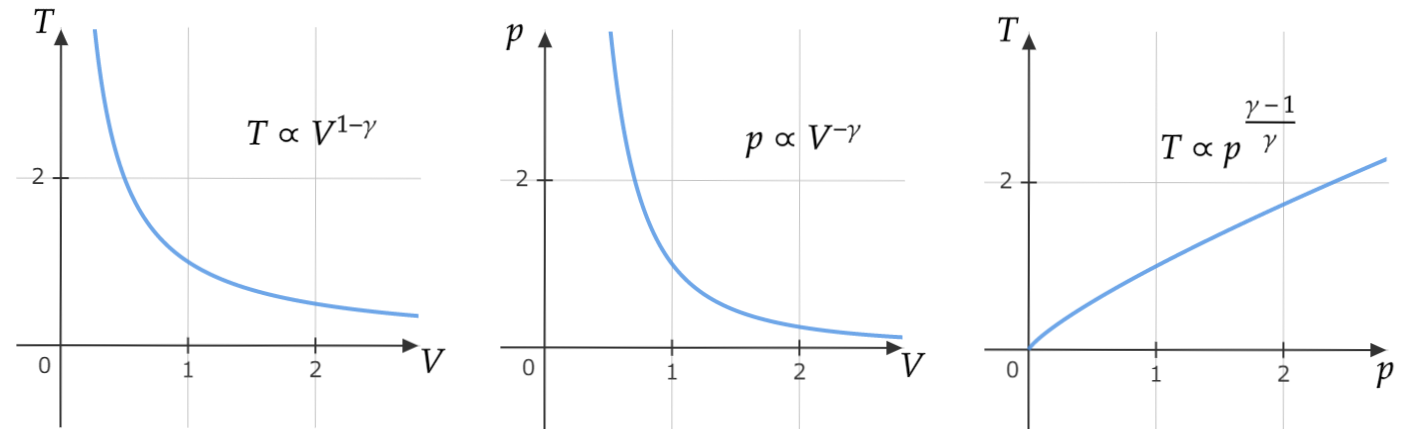
\includegraphics[scale = 0.4]{Images/AdiabaticIdealGas.png}
        \caption{Relationships for temperature, pressure, and volume for an adiabatic process involving an ideal gas.}
    \end{figure}
\end{eg}

Some specific applications of adiabatic processes are as follows: \begin{itemize}
    \item Diesel engine (spontaneous explosion due to heating; no spark plugs)
    \item Chinooks (air pressure increases due to lower altitude)
\end{itemize}



\begin{eg}[Black-body radiation]
    We now deal with electromagnetic radiation in a cavity in thermal equilibrium, which is emitted by black walls. Here ``black" means all radiation is absorbed:
    \begin{center}
        \begin{tikzpicture}[x=0.75pt,y=0.75pt,yscale=-1,xscale=1]
%uncomment if require: \path (0,398); %set diagram left start at 0, and has height of 398

%Shape: Rectangle [id:dp6362389483265465] 
\draw  [fill={rgb, 255:red, 253; green, 0; blue, 0 }  ,fill opacity=1 ][line width=2.25]  (100,126) -- (460,126) -- (460,306) -- (100,306) -- cycle ;
%Shape: Rectangle [id:dp03100105207175874] 
\draw  [color={rgb, 255:red, 0; green, 0; blue, 0 }  ,draw opacity=1 ][fill={rgb, 255:red, 255; green, 255; blue, 255 }  ,fill opacity=1 ][line width=2.25]  (190,171) -- (370,171) -- (370,261) -- (190,261) -- cycle ;

% Text Node
\draw (345,183.07) node [anchor=north west][inner sep=0.75pt]    {$V$};
% Text Node
\draw (443,280.07) node [anchor=north west][inner sep=0.75pt]    {$T$};
% Text Node
\draw (193,242.67) node [anchor=north west][inner sep=0.75pt]   [align=left] {Cavity};
% Text Node
\draw (102,286.67) node [anchor=north west][inner sep=0.75pt]   [align=left] {Heat Bath};


\end{tikzpicture}
    \end{center}
    Experiments show that $U = U(T,V) = V\epsilon(T)$, where $\epsilon$ is the energy density per volume. From classical electromagnetism, we also have $p = \frac{1}{3}\epsilon(T)$ for isotropic radiation (uniform radiation). The existence of a pressure from the classical perspective is similar to what we have for a gas. We can also borrow the wave-particle dualism from Quantum Mechanics. This suggests that we might be able to interpret or model black-body radiation as a \Emph{photon gas} (at least in a first approximation). Using our previous derivation for a gas we have \begin{equation*}
        C_V = \frac{\partial U}{\partial T} = V\frac{d\epsilon}{dT}
    \end{equation*}
    and for adiabats we find then \begin{equation*}
        \left(\frac{dT}{dV}\right)_{ad} = -\frac{p + \frac{\partial U}{\partial V}}{C_V} = -\frac{\frac{4}{3}\epsilon(T)}{V\frac{d\epsilon}{dT}}
    \end{equation*}
    We can rewrite this to obtain the simple ODE \begin{equation*}
        -\frac{d\epsilon}{\epsilon} = \frac{4}{3}\frac{dV}{V}
    \end{equation*}
    The solution of this ODE can be written as \begin{equation*}
        \epsilon V^{4/3} = const.
    \end{equation*}
    which has the equivalent form \begin{equation*}
        pV^{4/3} = const.
    \end{equation*}
    given the relationship between $p$ and $\epsilon$ for black-body radiation from above.
\end{eg}


Since no heat is flowing in or out of the system in an adiabatic process, in the absence of any friction we can completely recover the original state of the system by reversing the procedure. Such a process also converses entropy, as we will see later. 

\begin{defn}
    A thermodynamic process which is both adiabatic and reversible is said to be an \Emph{isentropic process}.
\end{defn}




\subsection{Isotherms}

\begin{defn}
    An \Emph{isotherm} is a change in the state of a system such that $dT = 0$.
\end{defn}

This is not to be confused with an adiabatic process in which there is no heat trnasfer between the surroundings and the system. $dT = 0$ relates to a level surface, or manifold, associated to a constant empirical temperature $\Theta$, which we use to define $T$.





%%%%%%%%%%%%%%%%%%%%%% Chapter 1.3
\chapter{Thermodynamical Potentials and Equilibrium}




%%%%%%%%%%%%%%%%%%%%%%%%%%%%%%%%%%%%% Part 2
\part{Statistical Mechanics}


%%%%%%%%%%%%%%%%%%%%%% Chapter 2.1
\chapter{Microstates and Entropy}



%%%%%%%%%%%%%%%%%%%%%% Chapter 2.2
\chapter{Ensemble Theory and Free Energy}



%%%%%%%%%%%%%%%%%%%%%% Chapter 2.3
\chapter{Boltzmann Statistics and the Canonical Ensemble}



%%%%%%%%%%%%%%%%%%%%%% Chapter 2.4
\chapter{Breakdown of Classical Statistical Mechanics}



%%%%%%%%%%%%%%%%%%%%%%%%%%%%%%%%%%%%% Part 3
\part{Probability Theory}


%%%%%%%%%%%%%%%%%%%%%% Chapter 3.1
\chapter{Characteristics of Probability Theory}


%%%%%%%%%%%%%%%%%%%%%% Chapter 3.2
\chapter{Continuous Random Variables and the Gaussian Distribution}


%%%%%%%%%%%%%%%%%%%%%% Chapter 3.3
\chapter{Information and Entropy}





%%%%%%%%%%%%%%%%%%%%%%%%%%%%%%%%%%%%% Part 4
\part{Real Gases and Phase Transitions}


%%%%%%%%%%%%%%%%%%%%%% Chapter 4.1
\chapter{Kinetic Theory of Gases}



%%%%%%%%%%%%%%%%%%%%%% Chapter 4.2
\chapter{Classification of Phase Transitions}






%%%%%%%%%%%%%%%%%%%%%%%%%%%%%%%%%%%%% Part 5
\part{Quantum Statistics}


%%%%%%%%%%%%%%%%%%%%%% Chapter 5.1
\chapter{Quantum States}


%%%%%%%%%%%%%%%%%%%%%% Chapter 5.2
\chapter{Ideal Quantum Gases}








%%%%%%%%%%%%%%%%%%%%%% - Appendices
\begin{appendices}


\end{appendices}


\end{document}


%%%%%% END %%%%%%%%%%%%%
